\documentclass[a4paper,oneside,12pt]{report}
\usepackage{styles/fbe_tez}
\usepackage[utf8x]{inputenc} % To use Unicode (e.g. Turkish) characters
\usepackage{amsmath, amsthm} % Some extra symbols
\usepackage{diagbox}
\usepackage[bottom]{footmisc}
\usepackage{cite}
\usepackage{graphicx}
\usepackage{longtable}
\usepackage{float}
\usepackage{multirow}
\usepackage{subfigure}
\usepackage{algorithm}
\usepackage{algorithmic}
\usepackage{array}
\usepackage{amssymb,bm,cite,graphicx, fixmath, texdraw}
\usepackage{epsfig}
\usepackage{epstopdf}
\usepackage{subfigure} % 
\usepackage{amsmath}
\usepackage{notoccite}
\usepackage[colorlinks=true, allcolors=blue]{hyperref}
\usepackage{grffile}
%%mehmet added
\usepackage{listings}
\usepackage{xcolor}

% SystemVerilog Definition
\lstdefinelanguage{SystemVerilog}[]{Verilog}{
  morekeywords={logic, always_ff, always_comb, always_latch, byte, shortint, int, longint, integer, time, bit, reg, enum, struct, union, interface, modport, package, import, export, program, property, sequence, assert, config, design, clocking, default, disable, endclocking, endconfig, endgroup, endinterface, endmodule, endpackage, endprimitive, endprogram, endproperty, endsequence, endtable, expect, generate, join_any, join_none, local, matches, pure, solve, super, this, virtual, wait_order, within, signed},
}

% Verilog-A Definition
\lstdefinelanguage{Verilog-A}[]{Verilog}{
  morekeywords={analog, discipline, electrical, voltage, current, ground, transition, laplace_nd, idt, ddt, white_noise, flicker_noise, analysis, cross, above, timer, initial_step, final_step},
}

% MATLAB Definition
\lstdefinelanguage{MATLAB}{
  morekeywords={break,case,catch,classdef,continue,else,elseif,end,for,function,global,if,otherwise,parfor,persistent,return,spmd,switch,try,while},
  sensitive=true,
  morecomment=[l]{\%},
  morecomment=[s]{\%\{}{\%\}},
  morestring=[m]',
}

\lstset{
    extendedchars=true,
    literate={Σ}{{$\Sigma$}}1 {Δ}{{$\Delta$}}1 {μ}{{$\mu$}}1 {°}{{$^\circ$}}1,
    basicstyle=\small\ttfamily,
    keywordstyle=\color{black}\bfseries, 
    commentstyle=\color{gray}\itshape,
    stringstyle=\color{black}, % Added to ensure MATLAB strings look clean
    numbers=none,
    frame=none,
    breaklines=true,
    xleftmargin=1.5em,
    showstringspaces=false, % Keeps MATLAB strings from having visible space symbols
}

\interdisplaylinepenalty=2500
\hyphenation{lists} \makeatletter

\newcommand{\field}[1]{\mathbb{#1} }
\newcommand{\beq}{\begin{equation} \setlength\abovedisplayskip{5pt} 
\setlength\belowdisplayskip{5pt}}
\newcommand{\eeq}{\end{equation}}
\newcommand{\bea}{\begin{eqnarray}}
\newcommand{\eea}{\end{eqnarray}}
\newcommand{\defn}{\stackrel{\triangle}{=}}
\newcommand{\nn}{\nonumber}
\newcommand{\nnl}{\nonumber \\}
\renewcommand{\theequation}{\arabic{equation}}
\renewcommand{\labelenumi}{(\roman{enumi})}

\DeclareMathOperator*{\argmin}{arg\,min}
\DeclareMathOperator*{\argmax}{arg\,max}

\def\ifundefined{\@ifundefined}
\def\bfat{\left[ \begin{array}}
\def\emat{\end{array} \right]}
\def\bfatt{\left\{ \begin{array}}
\def\ematt{\end{array} \right.}
\def\bset{\left\{ \begin{array}}
\def\eset{\end{array} \right\}}
\def\bpar{\left( \begin{array}}
\def\epar{\end{array} \right)}

\graphicspath{{figures/}} % Graphics will be here

\newtheorem{thm}{Theorem}[chapter]
\newtheorem{prop}[thm]{Proposition}
\newtheorem{lem}[thm]{Lemma}
\newtheorem{cor}[thm]{Corollary}

\numberwithin{equation}{chapter}

% COVER PAGE
\title{Modeling and Implementation of a Photovoltaic cell battery charger system}
\turkcebaslik{Fotovoltaik Hücre Batarya Şarj Sistemi Modelleme ve Uygulaması}
\degree{B.S., Electrical and Electronics Engineering, Boğaziçi University, 2020\\
	M.S., Electrical and Electronics Engineering, Boğaziçi University, 2026}
\author{Mehmet Gök}
\program{Electrical and Electronics Engineering}
\subyear{2026}

% APPROVED BY PAGE
\supervisor{Prof. Günhan Dündar}
%\cosuperi{Title and Name of Cosupervisor I}
%\cosuperii{Title and Name of Cosupervisor II}
\examineri{Assoc. Prof. Name Surname}
\examinerii{Assist. Prof. Name Surname}
\examineriii{Name Surname, Ph.D.}
%\examineriv{}
%\examinerv{}
\dateofapproval{DD.MM.YYYY}

% BEGIN OF DOCS
\begin{document}
\pagenumbering{roman}
\makemstitle % M.S. thesis
\makeapprovalpage

% ACK PAGE
\begin{acknowledgements}
I would like to express my deepest gratitude to my supervisor, Prof. Günhan Dündar, for his invaluable guidance and support throughout this research. I am also thankful to my family and friends for their unwavering encouragement and patience during this journey.
\end{acknowledgements}

% ABS PAGE
\begin{abstract}
This thesis presents the modeling and implementation of a photovoltaic cell battery charger system. The study focuses on the design of a fuzzy logic controller to optimize the charging process while ensuring maximum power point tracking (MPPT). Simulation and experimental results demonstrate the effectiveness of the proposed system in achieving high efficiency and reliability under varying conditions.
\end{abstract}

% OZET PAGE
\begin{ozet}
Bu tez, bir fotovoltaik hücre batarya şarj sisteminin modellenmesi ve uygulanmasını sunmaktadır. Çalışma, şarj işlemini optimize etmek ve maksimum güç noktası takibini (MPPT) sağlamak için bir bulanık mantık denetleyicisinin tasarımına odaklanmaktadır. Simülasyon ve deneysel sonuçlar, önerilen sistemin değişen koşullar altında yüksek verimlilik ve güvenilirlik sağlama konusundaki etkinliğini göstermektedir.
\end{ozet}

% CONTENTS AND LIST OF FIG AND TABLE PAGES
\tableofcontents
\listoffigures
\listoftables

% LIST OF SYMBOLS PAGE
\begin{symbols}
% The title will be typeset as "LIST OF SYMBOLS".
% Use a separate \sym command for each symbols definition.
% First, Latin symbols in alphabetical order
\sym{$V_{pv}$}{Photovoltaic panel output voltage}
\sym{$I_{pv}$}{Photovoltaic panel output current}
\sym{$P_{pv}$}{Photovoltaic panel output power}
\sym{$V_{b}$}{Battery voltage}
% 1 EMPTY LINE BETWEEN LATIN AND GREEK SYMBOLS GROUP!!!
\sym{}{}
% Then Greek symbols in alphabetical order
\sym{$\eta$}{Efficiency}
\sym{$\tau$}{Time constant}
\sym{$\Delta$}{Change or differential}
\sym{ }{}
\end{symbols}

% LIST OF ABBREV PAGE
\begin{abbreviations}
 % Abbreviations in alphabetical order
\sym{ADC}{Analog-to-Digital Converter}
\sym{CC}{Constant Current}
\sym{DAC}{Digital-to-Analog Converter}
\sym{FLC}{Fuzzy Logic Controller}
\sym{I-V}{Current-Voltage}
\sym{LDO}{Low Drop Out Regulator}
\sym{MPPT}{Maximum Power Point Tracking}
\sym{P-V}{Power-Voltage}
\sym{PV}{Photovoltaic}
\sym{PWM}{Pulse Width Modulation}
\sym{S/H}{Sample and Hold}
\sym{SoC}{State of Charge}
\sym{SPI}{Serial Peripheral Interface}
\end{abbreviations}

% MAIN CHAPTERS
\chapter{INTRODUCTION}
\label{chapter:introduction}
\pagenumbering{arabic}

\section{Renewable Energy and Photovoltaic Systems}
\label{sec:intro_renewable}
The global demand for energy is rising rapidly, driven by population growth and industrialization. Concurrently, environmental concerns regarding fossil fuels have accelerated the transition towards renewable energy sources. Among these, solar energy stands out as a clean, abundant, and sustainable resource. Photovoltaic (PV) systems, which convert sunlight directly into electricity using semiconductor materials, have become a dominant technology in the renewable energy sector.

However, the efficiency of energy conversion in PV systems is heavily dependent on environmental conditions. The power output of a PV panel is non-linear and varies significantly with solar irradiance and ambient temperature. Unlike conventional power sources, a PV array does not have a constant internal impedance. Consequently, to extract the maximum available power, the load impedance must be dynamically matched to the source impedance. This necessity leads to the implementation of Maximum Power Point Tracking (MPPT) controllers.

\section{Maximum Power Point Tracking Algorithms}
\label{sec:intro_mppt_techniques}
Maximum Power Point Tracking (MPPT) is a critical technique in photovoltaic (PV) systems used to maximize power extraction under all conditions. The P-V characteristic of a solar panel is non-linear and varies with solar irradiance and temperature. There is a unique point on the P-V curve, known as the Maximum Power Point (MPP), where the PV system produces maximum power. MPPT algorithms adjust the electrical operating point of the modules to keep them at the MPP. Several algorithms have been developed to achieve this, varying in complexity, sensor requirements, convergence speed, and cost.

\subsection{Perturb and Observe (P\&O)}
The Perturb and Observe (P\&O) algorithm is one of the most widely used methods due to its simplicity and ease of implementation. It operates by periodically perturbing (increasing or decreasing) the terminal voltage of the PV array and comparing the PV output power with that of the previous cycle. If the power increases, the perturbation is continued in the same direction. If the power decreases, the direction is reversed. While simple, P\&O suffers from oscillations around the MPP in steady state and can track in the wrong direction during rapidly changing atmospheric conditions.

\subsection{Incremental Conductance (IncCond)}
The Incremental Conductance (IncCond) method is based on the fact that the slope of the PV array power curve is zero at the MPP, positive on the left of the MPP, and negative on the right. It compares the instantaneous conductance ($I/V$) with the incremental conductance ($dI/dV$). Although IncCond offers better tracking accuracy and stability compared to P\&O, particularly under rapidly changing conditions, it requires more complex control circuitry and higher computational power.

\subsection{Fuzzy Logic Control (FLC)}
Fuzzy Logic Control (FLC) has emerged as a powerful alternative for MPPT, especially in systems where the mathematical model is difficult to derive or is highly non-linear. FLC operates based on linguistic rules and does not require precise knowledge of the system parameters. It is robust against parameter variations and environmental noise. Compared to P\&O and IncCond, FLC offers faster convergence and reduced oscillations around the MPP, making it highly suitable for battery charging applications where efficiency and battery health are paramount.

\section{Proposed Solution}
\label{sec:intro_proposed_system}
Based on the comparison of MPPT techniques presented in the previous section, this thesis proposes a photovoltaic battery charger system that employs a Fuzzy Logic Controller (FLC). While P\&O is simple, it suffers from oscillations, and IncCond, while accurate, is computationally intensive. FLC offers a balance of robustness, fast convergence, and adaptability to the non-linear characteristics of PV panels without requiring complex mathematical modeling.

The proposed system integrates the PV panel with a DC-DC buck converter controlled by the FLC algorithm to charge a battery efficiently. This approach ensures optimal energy harvesting even under rapidly changing atmospheric conditions.

\begin{figure}[H]
    \centering
    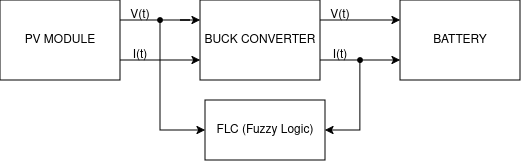
\includegraphics[width=0.8\textwidth]{introduction/system_overview.drawio.png}
    \caption{Fuzzy Logic PV Charger Overview.}
    \label{fig:intro_system_overview}
\end{figure}

\chapter{MATLAB MODEL}
\label{chapter:matlab_model}

\section{MATLAB Model Overview}
\label{sec:matlab_overview}
The design and verification of the proposed photovoltaic battery charger system were initially conducted using the MATLAB/Simulink environment. Simulink provides a comprehensive platform for Model-Based Design, allowing for the simulation of complex dynamic systems before physical implementation.

One of the primary advantages of using Simulink for this application is the availability of the Simscape Electrical library. This library offers pre-built, high-fidelity models for power electronic components, such as MOSFETs, diodes, inductors, and capacitors, as well as specialized sources like the Photovoltaic Array block. The built-in PV array model allows for precise definition of the panel's characteristics and enables the simulation of varying environmental conditions, such as changes in solar irradiance and temperature, which are crucial for testing MPPT algorithms.

Furthermore, MATLAB's Fuzzy Logic Toolbox facilitates the design and visualization of the Fuzzy Inference System (FIS). This toolbox allows for the intuitive definition of membership functions and rules, which can then be directly integrated into the Simulink simulation via the Fuzzy Logic Controller block. This integration enables rapid prototyping and tuning of the control parameters to achieve optimal tracking performance and stability.

\begin{figure}[H]
    \centering
    
\includegraphics[width=0.8\textwidth]{matlab/matlab_model_overview.png}
    \caption{MATLAB Model Block Diagram.}
    \label{fig:matlab_model_block_diagram}
\end{figure}

\section{Photovoltaic Cell Model}
\label{sec:matlab_pv_model}
A fundamental component of the proposed system is the photovoltaic (PV) cell, which converts solar energy into electrical energy. To accurately simulate and control the charging process, a mathematical model representing the PV cell's behavior is essential. This section details the model used, specifically focusing on its non-linear current-voltage (I-V) and power-voltage (P-V) characteristics.

The output power of a PV panel is not constant; it varies significantly with environmental conditions, primarily solar irradiance and temperature. As shown in the P-V characteristics, there exists a single operating point for any given set of conditions where the power extraction is maximized. This point is referred to as the Maximum Power Point (MPP). Because the location of the MPP shifts as irradiance or temperature changes, a static connection between the panel and the load is inefficient. Therefore, it is imperative to employ Maximum Power Point Tracking (MPPT) techniques. MPPT ensures that the load impedance seen by the source is adjusted to match the optimal operating point, thereby maximizing the efficiency of energy harvesting.

Figure \ref{fig:pv_curves} illustrates the I-V and P-V characteristics of the modeled PV cell. The plot explicitly displays curves for three different irradiance levels, highlighting how the short-circuit current and the maximum power point scale with the intensity of the incident sunlight.

\begin{figure}[H]
    \centering
    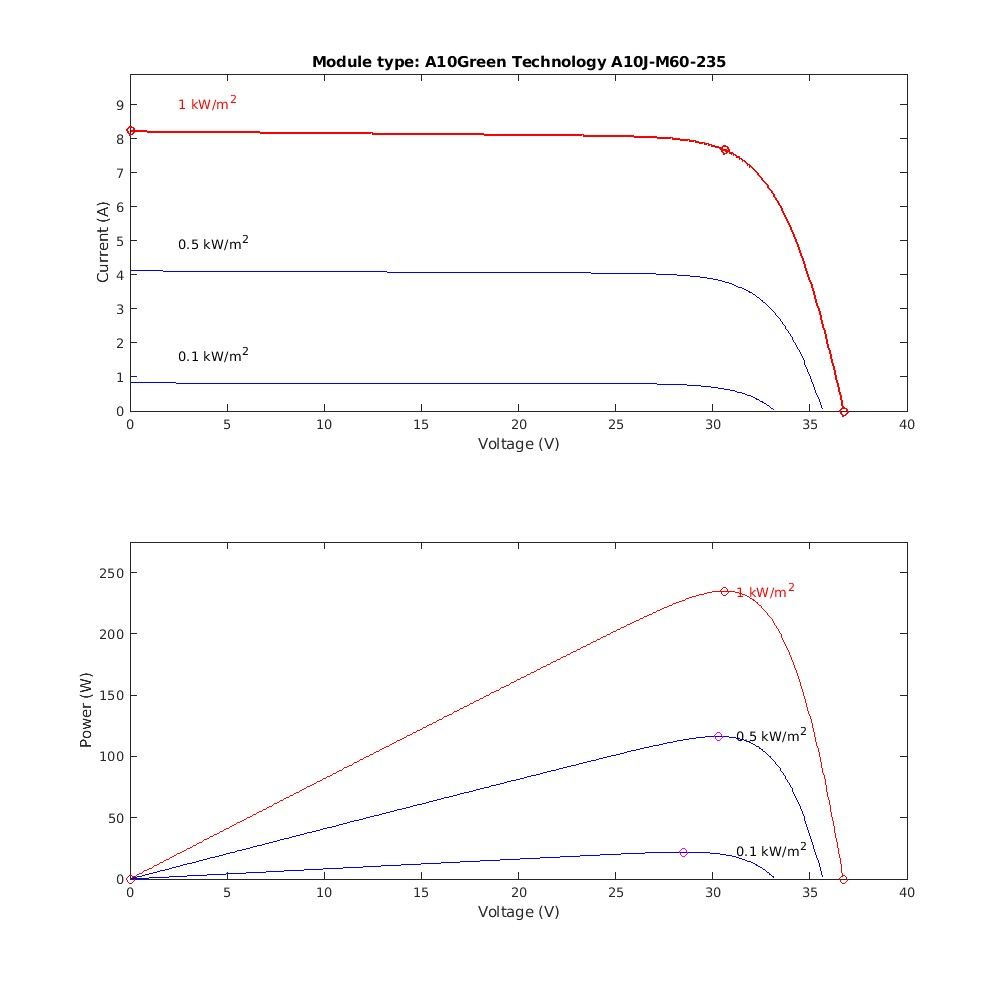
\includegraphics[width=0.8\textwidth]{introduction/pv_IV&powercurves.jpg}
    \caption{PV Cell I-V and P-V Characteristics.}
    \label{fig:pv_curves}
\end{figure}

\section{Buck Converter}
\label{sec:matlab_buck_converter}
The buck converter is a fundamental DC-DC topology used to step down a higher input voltage to a lower output voltage while maintaining high efficiency. It operates by chopping the input voltage using a controlled switch (typically a MOSFET) and filtering the resulting signal with an inductor and a capacitor. The ratio of the output voltage to the input voltage is primarily determined by the duty cycle of the switch.

In this specific application, the photovoltaic panel operates at a Maximum Power Point (MPP) voltage of approximately 30 V. However, the system is designed to charge a 12 V battery. Consequently, a buck converter is employed to bridge this voltage difference. This configuration not only steps down the voltage but also allows the MPPT algorithm to adjust the effective load impedance seen by the PV panel by varying the duty cycle, thereby maximizing power extraction.

The design parameters for the buck converter, as defined in the system's MATLAB model, are presented in Table \ref{tab:buck_params}. These specifications are derived based on the design guidelines and component selection criteria described in \cite{EricksonBook, RashidBook, TIReport}.

\begin{table}[H]
    \centering
    \caption{Buck Converter Specifications}
    \begin{tabular}{|l|c|c|}
        \hline
        \textbf{Parameter} & \textbf{Symbol} & \textbf{Value} \\
        \hline
        Input Voltage (MPP) & $V_{in}$ & 30.6 V \\
        \hline
        Output Voltage (Battery) & $V_{out}$ & 14.4 V \\
        \hline
        Switching Frequency & $f_{sw}$ & 500 kHz \\
        \hline
        Inductance & $L$ & 2.6 $\mu$H \\
        \hline
        Input Capacitance & $C_{in}$ & 47 $\mu$F \\
        \hline
    \end{tabular}
    \label{tab:buck_params}
\end{table}

\section{Fuzzy Logic Controller}
\label{sec:matlab_flc}
To address the non-linear characteristics of the PV array and the need for robust tracking under changing environmental conditions, this thesis employs a Fuzzy Logic Controller (FLC). Unlike traditional linear controllers, the FLC does not require an exact mathematical model of the plant, making it highly effective for the time-varying nature of solar irradiance and temperature.

The control algorithm is based on a Sugeno-type fuzzy inference system, which is chosen for its computational efficiency and its suitability for generating a crisp control output, making it well-suited for digital implementation in control systems. The overall process of the FLC can be divided into three main stages: sampling, rule firing, and duty adjustment.

\begin{figure}[H]
    \centering
    
\includegraphics[width=0.8\textwidth]{matlab/fuzzy_controller_block_diagram.png}
    \caption{Fuzzy Logic Controller Block Diagram.}
    \label{fig:fuzzy_controller_block_diagram}
\end{figure}

\subsection{Sampling}
The controller is implemented digitally with a sampling frequency of 20 kHz, as defined in the system parameters. At each sampling instant, the controller reads the PV voltage and current. The ADCs used for this purpose have a 10-bit resolution, which provides $2^{10} = 1024$ discrete levels (counts) to represent the analog signals. This allows for a fine-grained measurement of the PV voltage and current, which is essential for the accuracy of the MPPT algorithm. This sampling frequency is chosen to be sufficiently lower than the 500 kHz switching frequency to avoid aliasing while maintaining a fast transient response. 

\subsection{Rule Firing}
The core of the FLC is the rule firing stage, where the necessary change in the duty cycle ($\Delta D$) is determined based on the sampled inputs. This stage processes three key inputs:
\begin{enumerate}
    \item \textbf{Change in PV Voltage ($dV$):} The difference in the PV voltage reading between consecutive samples.
    \item \textbf{Change in PV Current ($dI$):} The difference in the PV current reading between consecutive samples.
    \item \textbf{PV Voltage ($V_{pv}$):} The instantaneous PV voltage, used to determine the operating region of the PV panel.
\end{enumerate}

The process involves three steps:
\begin{itemize}
    \item \textbf{Fuzzification:} The crisp input values are converted into linguistic variables (e.g., Negative, Zero, Positive for $dV$ and $dI$; \texttt{Low\textunderscore Voltage}, \texttt{Optimal\textunderscore Range}, \texttt{High\textunderscore Voltage} for $V_{pv}$) using linear and triangular membership functions.
    \item \textbf{Rule Evaluation:} A set of linguistic rules is evaluated to determine the control action. The rule base, summarized in Tables \ref{tab:fuzzy_rules_safety} and \ref{tab:fuzzy_rules_optimal}, is divided into two main groups: safety rules that make large adjustments when the voltage is too low or too high, and fine-tuning rules for operation near the MPP. A critical rule is that if both $dV$ and $dI$ are zero, the duty cycle is held constant to prevent oscillations at the power peak.
    \item \textbf{Defuzzification:} The output of the Sugeno system is a set of constant values for the change in duty cycle ($\Delta D$), such as \texttt{Big\textunderscore Decrease} (-15), \texttt{Decrease} (-1), \texttt{Hold} (0), \texttt{Increase} (+1), and \texttt{Big\textunderscore Increase} (+15). The final output is a weighted average of the active rule outputs.
\end{itemize}

These rules provide a two-tiered control strategy. The safety rules (Table \ref{tab:fuzzy_rules_safety}) trigger when the PV voltage moves into the \texttt{Low\textunderscore Voltage} or \texttt{High\textunderscore Voltage} regions. These regions are defined by membership functions in the fuzzy inference system, as specified in the \texttt{matlab\_code/create\_mppt\_fis.m} script. With a 10-bit ADC and a 40V reference, the conversion from a voltage $V$ to an ADC count is given by: $ADC_{count} = (V / 40V) \times 1024$.

The MPP for the modeled panel is at 30.6V (approx. ADC count 783). The safety rules are configured for large deviations from this point. For instance, the \texttt{Low\textunderscore Voltage} membership function (see \texttt{create\_mppt\_fis.m}) becomes fully active for ADC counts below 730. This corresponds to a voltage of approximately 28.5V, calculated as $(730 / 1024) \times 40V$. If the panel voltage drops into this region, the controller applies a \texttt{Big\textunderscore Decrease} to the duty cycle, raising the panel voltage back towards the MPP. Conversely, the \texttt{High\textunderscore Voltage} membership function begins to activate at an ADC count of 840, which corresponds to 32.8V ($(840 / 1024) \times 40V$). If the voltage exceeds this, the controller applies a \texttt{Big\textunderscore Increase} to lower the panel voltage.

Once the voltage is within the \texttt{Optimal\textunderscore Range}, the fine-tuning rules take over, making small adjustments to zero in on the precise MPP and hold it there, as detailed in Table \ref{tab:fuzzy_rules_optimal}.

\subsection{Duty Adjustment}
The final stage is the adjustment of the duty cycle. To ensure a smooth transition between different control states and prevent abrupt changes in the duty cycle, a bumpless transfer mechanism is implemented. This is achieved by taking the duty cycle output from the general duty cycle register ($D[n-1]$) and adding the calculated change ($\Delta D$). This feedback loop ensures that the control signal evolves continuously from the previous state, preventing discontinuities when switching between loop dynamics.

Additionally, the integrator and the scaling of the output provide a damping effect. This lowers the impact of abrupt changes, reducing oscillations and making the system robust against noise and environmental disturbances. In the MATLAB model, the calculated $\Delta D$ is divided by a gain factor (e.g., 16384). This ``lowering effect'' reduces the magnitude of the duty cycle adjustments, allowing for very fine control granularity in the continuous simulation environment.

\begin{table}[H]
    \centering
    \caption{Fuzzy Logic Safety Rules}
    \begin{tabular}{|c|c|}
        \hline
        \textbf{PV Voltage ($V_{pv}$)} & \textbf{Output ($\Delta D$)} \\
        \hline
        \texttt{Low\textunderscore Voltage} & \texttt{Big\textunderscore Decrease} \\
        \hline
        \texttt{High\textunderscore Voltage} & \texttt{Big\textunderscore Increase} \\
        \hline
    \end{tabular}
    \label{tab:fuzzy_rules_safety}
\end{table}

\begin{table}[H]
    \centering
    \caption{Fuzzy Logic Rules for Optimal Range}
    \begin{tabular}{|c|c|c|c|}
        \hline
        \diagbox{$dI$}{$dV$} & \textbf{Negative} & \textbf{Zero} & \textbf{Positive} \\
        \hline
        \textbf{Negative} & \texttt{Decrease} & \texttt{Hold} & \texttt{Increase} \\
        \hline
        \textbf{Zero} & Not Defined & \texttt{Hold} & Not Defined \\
        \hline
        \textbf{Positive} & \texttt{Increase} & \texttt{Hold} & \texttt{Decrease} \\
        \hline
    \end{tabular}
    \label{tab:fuzzy_rules_optimal}
\end{table}

\section{Simulation Results}
\label{sec:matlab_sim_results}
The performance of the proposed fuzzy logic-based MPPT controller was validated through a comprehensive simulation conducted in MATLAB/Simulink, with the overall results depicted in Figure \ref{fig:matlab_sim_result}. The total simulation time was 0.6 seconds, designed to demonstrate the controller's performance during both steady-state and transient conditions. The converter efficiency, calculated as $P_{out}/P_{in}$, was maintained at approximately 95\% throughout the simulation. The PV efficiency, defined as $P_{in}/P_{vmax}$, is the primary metric for evaluating the MPPT algorithm's effectiveness.

The simulation is divided into three distinct phases, with the critical transient moments highlighted in detail in Figure \ref{fig:matlab_sim_zooms}.

\begin{enumerate}
    \item \textbf{Initial Stabilization (0s - 0.2s):} For the first 0.2 seconds, the system operates with a fixed duty cycle. The fuzzy logic controller is inactive, allowing the converter to stabilize without active MPPT control, as seen in the first section of Figure \ref{fig:matlab_sim_result}.

    \item \textbf{Fuzzy Controller Activation (0.2s):} At 0.2 seconds, the fuzzy logic MPPT controller is enabled. Figure \ref{fig:sim_zoom_02} shows a zoomed-in view of this event. The controller rapidly adjusts the duty cycle to find the maximum power point, achieving over 99\% PV efficiency in just 13.4 milliseconds, which highlights its fast convergence speed.

    \item \textbf{Transient Response (0.4s):} At 0.4 seconds, a step change simulates a sudden decrease in solar irradiance. Figure \ref{fig:sim_zoom_04} details this transient. Despite the disturbance causing a momentary dip in PV efficiency to 90\%, the fuzzy controller responds swiftly, restoring the efficiency to over 99\% in approximately 1 millisecond.
\end{enumerate}

These results confirm the robustness and high performance of the fuzzy logic controller, showcasing its ability to quickly track the MPP and maintain high efficiency, even under rapidly changing conditions.

\begin{figure}[H]
    \centering
    
\includegraphics[width=0.9\textwidth]{matlab/matlabsimresult.jpg}
    \caption{Overall MATLAB simulation results showing the three performance phases.}
    \label{fig:matlab_sim_result}
\end{figure}

\begin{figure}[H]
    \centering
    \subfigure[Zoomed-in view of FLC activation at 0.2s.]{
\includegraphics[width=0.7\textwidth]{matlab/matlab_sim_result_around0_2.jpg}\label{fig:sim_zoom_02}}
    \vfill
    \subfigure[Zoomed-in view of transient response at 0.4s.]{
\includegraphics[width=0.7\textwidth]{matlab/matlab_sim_result_around0_4.jpg}\label{fig:sim_zoom_04}}
    \caption{Zoomed-in views of transient events.}
    \label{fig:matlab_sim_zooms}
\end{figure}

\chapter{CADENCE MODEL IMPLEMENTATION}
\label{chapter:systemverilog}

The initial design and verification of the fuzzy logic controller were conducted in the MATLAB/Simulink environment, as detailed in Chapter 2. While MATLAB provides a powerful platform for algorithmic development and system-level simulation, the ultimate goal is to create a physical integrated circuit. To move towards a silicon-compatible implementation, the validated model must be migrated from the abstract, high-level MATLAB environment to a hardware description language (HDL) and simulated in an environment that supports circuit-level design and verification, such as Cadence. This chapter details the process of this migration, covering the implementation of the core components in SystemVerilog and Verilog-A, and the verification of the complete system within the Cadence Virtuoso platform.

\begin{figure}[H]
    \centering
    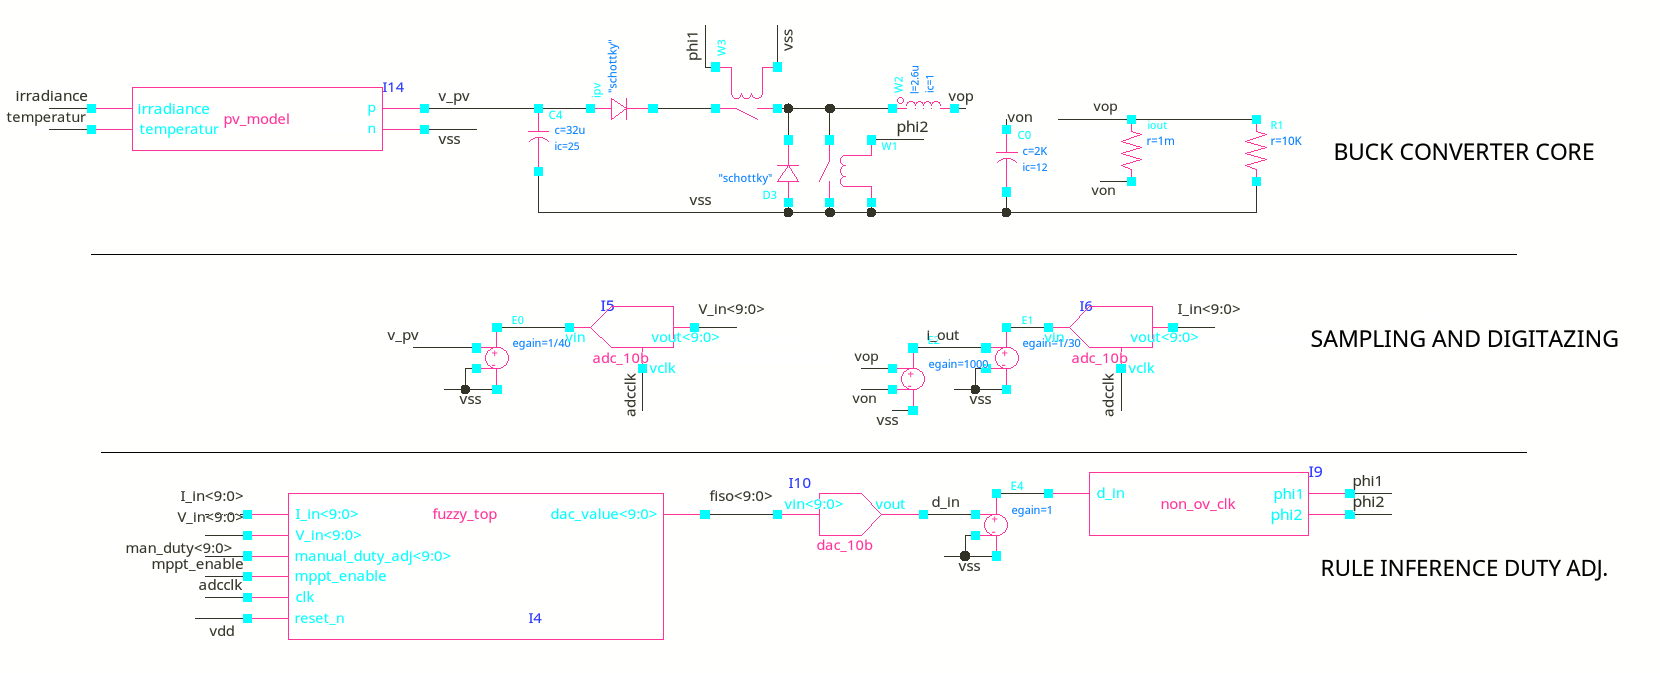
\includegraphics[width=0.8\textwidth]{figures/cadence_model/cadence_system_model.png}
    \caption{System Layout in Cadence.}
    \label{fig:cadence_layout}
\end{figure}

The overall system layout for the Cadence implementation is shown in Figure \ref{fig:cadence_layout}. While some components of the system, such as the ADCs, DACs, and the power switches of the buck converter, are based on standard and well-understood designs, their detailed implementation is not the focus of this chapter. Instead, the following subsections will focus on the more complex and non-straightforward parts of the design: the implementation of the fuzzy inference engine in SystemVerilog and the behavioral modeling of the PV panel in Verilog-A.

\section{PV Model Implementation in Verilog-A}
\label{sec:sv_pv_model}
To create a realistic simulation environment in Cadence, the photovoltaic panel was modeled using Verilog-A. This behavioral model replicates the non-linear I-V and P-V characteristics of the PV cell, allowing for accurate simulation of its interaction with the digitally-controlled buck converter. The model is based on the same mathematical equations used in the MATLAB simulation.

A widely recognized method for modeling PV panels is the five-parameter model, which uses a simplified equivalent circuit to predict the I-V curve. A significant contribution in this area was made by De Soto et al. \cite{DeSoto2006}, who developed and validated a method to determine the five key parameters (light-generated current $I_L$, diode saturation current $I_0$, ideality factor $n$, series resistance $R_s$, and shunt resistance $R_{sh}$) from standard manufacturer datasheet values. This approach allows for accurate performance prediction across a wide range of operating conditions (irradiance and temperature), which is essential for testing MPPT algorithms.

The Verilog-A implementation, shown below, is based on this five-parameter model. It takes irradiance and temperature as inputs and dynamically calculates the panel's output current based on its terminal voltage, accurately reproducing the non-linear behavior of the PV cell.

\lstinputlisting[language=Verilog-A, caption={Verilog-A PV Model Implementation}]{verilogacode/pv_model}

The Verilog-A code provides a behavioral model of the PV cell. Figure \ref{fig:pvmodel_ivandpower} shows the I-V (current-voltage) and P-V (power-voltage) characteristics produced by this model, highlighting the Maximum Power Point (MPP).

\begin{figure}[H]
    \centering
    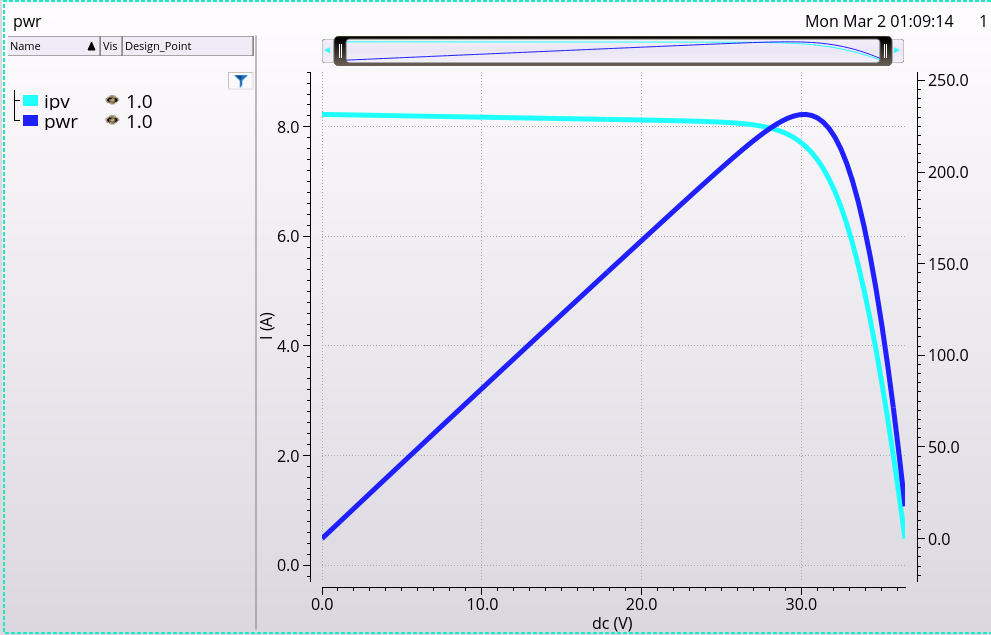
\includegraphics[width=0.8\textwidth]{cadence_model/pvmodel_ivandpower.png}
    \caption{I-V and P-V Characteristics of the Verilog-A PV Model.}
    \label{fig:pvmodel_ivandpower}
\end{figure}

While the MATLAB/Simulink model serves as the ideal reference, the Verilog-A behavioral model implemented in Cadence exhibits slight deviations in the electrical characteristics. These minor discrepancies arise from the implementation of the five-parameter equations and the analog solver's interpretation. Table \ref{tab:pv_model_comparison} compares the key parameters of the MATLAB reference model and the Verilog-A implementation.

\begin{table}[H]
    \centering
    \caption{Comparison of PV Model Parameters}
    \begin{tabular}{|l|c|c|}
        \hline
        \textbf{Parameter} & \textbf{MATLAB Model} & \textbf{Verilog-A Model} \\
        \hline
        Open Circuit Voltage ($V_{oc}$) & 36.72 V & 36.5 V \\
        \hline
        Short Circuit Current ($I_{sc}$) & 8.23 A & 8.226 A \\
        \hline
        MPP Voltage ($V_{mpp}$) & 30.6 V & 30.29 V \\
        \hline
        Maximum Power ($P_{mpp}$) & 235.008 W & 231.4 W \\
        \hline
    \end{tabular}
    \label{tab:pv_model_comparison}
\end{table}

\section{Fuzzy Logic Controller}
\label{sec:sv_fuzzy_engine}
To prepare the design for hardware implementation, the fuzzy logic controller, previously validated in MATLAB, was implemented as a digital module using SystemVerilog. SystemVerilog is a hardware description and verification language that allows for the creation of synthesizable logic, providing a direct path to a physical integrated circuit. This implementation follows a Sugeno-type fuzzy inference model, which is well-suited for hardware due to its computational efficiency. The process is broken down into three fundamental stages: fuzzification, inference, and defuzzification.

\subsection{Fuzzification}
\label{sec:sv_fuzzification}
In the fuzzification stage, the crisp digital inputs from the ADCs, representing the PV panel's voltage ($V_{pv}$) and current ($I_{pv}$), are converted into fuzzy linguistic variables. This is achieved by evaluating their degree of membership in predefined sets (e.g., `Low`, `Optimal`, `High`).

The core of this process is the calculation of the membership degree for a given input value. For this controller, triangular membership functions are used, which are defined by three points. A triangular function is composed of two linear segments, meaning the membership degree can be calculated using the simple equation of a line. If the slope and two points of a line are known, any other point is easily calculable.

Given two points $(x_1, y_1)$ and $(x_2, y_2)$, the slope ($m$) of the line connecting them is:
\begin{equation}
    m = \frac{y_2 - y_1}{x_2 - x_1}
\end{equation}
With the slope and a known point, the membership degree ($y$) for any input ($x$) can be calculated using the point-slope formula:
\begin{equation}
    y - y_1 = m(x - x_1)
\end{equation}
This linear relationship makes the calculation straightforward to implement in hardware, as shown in the SystemVerilog code below.
\lstinputlisting[caption={MF triangle SystemVerilog Implementation}, label={code:mf_triangle}]{systemverilogcode/mf_triangle.sv}
Other common membership functions, such as the linear S-shaped and Z-shaped functions, are similarly simple to implement in hardware as they are also based on linear equations.

\subsection{Inference}
\label{sec:sv_inference}
The inference engine serves as the decision-making core of the controller. It evaluates the fuzzy inputs generated in the fuzzification stage against the linguistic rules defined in the system's rule base. For this implementation, the logical 'AND' operator connecting the antecedents of a rule is realized using the minimum function, a standard method in fuzzy logic control.

Mathematically, for a rule with multiple conditions, such as:
\begin{equation}
    \text{IF } x \text{ is } A \text{ AND } y \text{ is } B \text{ THEN } z \text{ is } C
\end{equation}
The firing strength $w$ of the rule is calculated as:
\begin{equation}
    w = \min(\mu_A(x), \mu_B(y))
\end{equation}

In the SystemVerilog implementation, this logic is synthesized using combinational circuits. A dedicated function, \texttt{min3}, is created to compute the minimum of three values, facilitating rules that depend on $dV$, $dI$, and the $V_{pv}$ operating range simultaneously. The code below illustrates the parallel evaluation of the safety rules and the fine-tuning rules. The safety rules ($w_1, w_2$) are triggered solely by the PV voltage level, while the fine-tuning rules ($w_3$ to $w_8$) are active only when the voltage is within the optimal range, ensuring precise tracking around the MPP. This implementation strictly adheres to the logic defined in Tables \ref{tab:fuzzy_rules_safety} and \ref{tab:fuzzy_rules_optimal}.

\lstinputlisting[caption={Inference SystemVerilog Implementation}, label={code:inference}]{systemverilogcode/inference.sv}

As can be seen in the \texttt{always\_comb} block, the logic directly maps to the rule tables. The safety rules (w[1] and w[2]) depend only on the PV voltage, while the fine-tuning rules (w[3] through w[8]) are active only in the optimal voltage range (\texttt{Vpv\_mu\_opt}) and correctly implement the logic described in Table \ref{tab:fuzzy_rules_optimal}.

\subsection{Defuzzification}
\label{sec:sv_defuzzification}
The final stage of the fuzzy logic controller is defuzzification, which converts the fuzzy conclusions from the inference engine into a crisp, numerical control signal. Since this system utilizes a Sugeno-type inference model, the output membership functions are singletons (constant values) rather than distributed fuzzy sets. This simplifies the defuzzification process to a weighted average calculation, which is computationally efficient for hardware implementation.

The crisp output, representing the required change in duty cycle ($\Delta D$), is calculated using the Center of Gravity (CoG) method for singletons:
\begin{equation}
    \Delta D = \frac{\sum_{i=1}^{N} w_i \cdot C_i}{\sum_{i=1}^{N} w_i}
\end{equation}
where $w_i$ is the firing strength of the $i$-th rule, $C_i$ is the constant output value associated with that rule, and $N$ is the total number of rules.

The SystemVerilog implementation, shown below, defines the singleton constants corresponding to the linguistic variables \texttt{Big\textunderscore Decrease} (-15), \texttt{Decrease} (-1), \texttt{Hold} (0), \texttt{Increase} (+1), and \texttt{Big\textunderscore Increase} (+15). The module accumulates the weighted sum (numerator) and the total weight (denominator) to compute the final integer division.

\lstinputlisting[caption={defuzzification SystemVerilog Implementation}, label={code:defuzz}]{systemverilogcode/defuzzifier.sv}
\subsection{Duty Integration and Bumpless Transfer}
\label{sec:sv_duty_integrator}
The final stage of the digital control loop is the Duty Integrator. While the fuzzy inference engine determines the required \textit{change} in the operating point ($\Delta D$), the Pulse Width Modulation (PWM) generator requires an absolute duty cycle value to drive the power MOSFETs. This module performs the discrete-time integration of the fuzzy output, mathematically represented as:
\begin{equation}
    D[n] = D[n-1] + \Delta D[n]
\end{equation}
where $D[n]$ is the current duty cycle and $\Delta D[n]$ is the adjustment calculated by the defuzzifier.

This integration strategy serves two critical purposes:
\begin{enumerate}
    \item \textbf{Bumpless Transfer:} We take the duty cycle output from the general duty cycle register ($D[n-1]$) as the baseline. By adding the calculated change ($\Delta D$) to this existing global output, the system ensures a smooth transition. This prevents discontinuities that would otherwise occur when switching between different control dynamics (e.g., Safety vs. Fine-Tuning).
    \item \textbf{Robustness and Damping:} The integrator and damping provide the opportunity to lower oscillations and make the system robust. In the MATLAB model, this was achieved by dividing the output by a large gain factor. In the SystemVerilog implementation, where integer arithmetic prevents such division (as it would result in zero), this damping is achieved by accumulating small integer steps ($\pm 1, \pm 15$) into the high-resolution duty cycle register. This effectively lowers the impact of individual control actions, filtering out transient noise and maintaining stability around the MPP.
\end{enumerate}

The SystemVerilog implementation, provided below, includes saturation logic to constrain the duty cycle within safe hardware limits. It takes the signed 8-bit output from the defuzzifier and updates the 10-bit duty cycle register on every clock cycle.

\lstinputlisting[caption={Duty Integrator SystemVerilog Implementation}, label={code:duty_int}]{systemverilogcode/duty_integrator.sv}

It is important to note that the SystemVerilog code snippets provided in this section primarily serve to demonstrate the functional behavior and the algorithmic logic of the controller within the Cadence simulation environment. Direct implementation of arithmetic operations such as division---used here for the center-of-gravity defuzzification---can consume excessive logic resources and timing budget during synthesis. In a practical hardware implementation, these operations are often optimized or approximated using shifts, look-up tables, or specific architectural constraints to minimize area and power. Further details on the optimized digital implementation and synthesis considerations are discussed in Chapter \ref{chapter:digital_impl}.

\section{Simulation Results}
\label{sec:sv_simulation_results}
The functional verification of the SystemVerilog implementation was performed within the Cadence Virtuoso environment. The simulation was run for 180 ms, with the MPPT enabled at 0.3 ms.

As discussed in the duty integrator section, the selection of the damping fraction is critical. A fraction of 6 was selected; a higher value (e.g., 15) would result in excessive settling time for transient ringing. To further stabilize the inputs, $V_{pv}$, $I_{pv}$, and $I_{out}$ are processed through a moving average block with a window width of 200 $\mu$s.

Figure \ref{fig:cadence_results} illustrates the system's response. The extracted input power ($P_{in}$) settles at 227 W, which is close to the theoretical maximum of 231.4 W listed in Table \ref{tab:pv_model_comparison}. The average PV voltage ($V_{pv\_avg}$) stabilizes at 30.48 V, compared to the theoretical MPP voltage of 30.29 V. The output power ($P_{out}$) is measured at 217 W. This results in a PV efficiency ($P_{in}/P_{vmax}$) of $227/231.4 \approx 98.1\%$ and a converter efficiency ($P_{out}/P_{in}$) of $217/227 \approx 95.6\%$. Despite these minor deviations, the model demonstrates robust operation and successful tracking.

\begin{figure}[H]
    \centering
    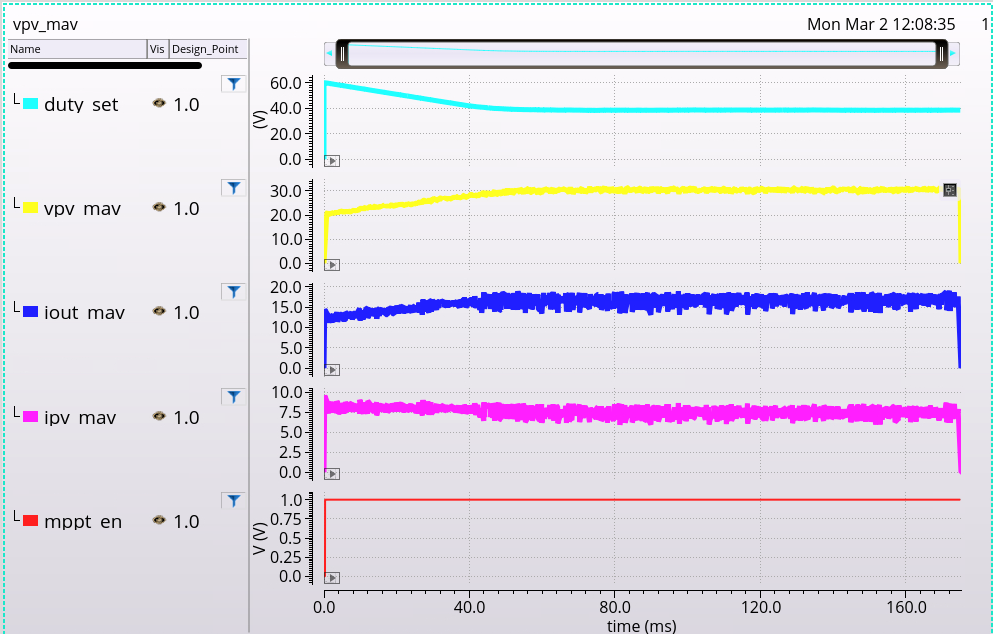
\includegraphics[width=0.8\textwidth]{figures/cadence_model/cadence_sim_result.png}
    \caption{Cadence Mixed-Signal Simulation Results showing MPP Tracking.}
    \label{fig:cadence_results}
\end{figure}

\section{System Block Diagram}
\label{sec:arch_block_diagram}
The complete system architecture integrates the digital control logic with the analog power and sensing components. Figure \ref{fig:system_block_diagram} illustrates the detailed block diagram, showing the signal flow from the PV panel sensors through the mixed-signal interface to the Fuzzy Logic Controller, and the resulting control signal driving the Buck Converter.

\begin{figure}[H]
    \centering
    
\includegraphics[width=1.0\textwidth]{{figures/cadence_model/Cadence_model.drawio}.png}
    \caption{System Block Diagram.}
    \label{fig:system_block_diagram}
\end{figure}

To ensure precise tracking and stable operation, the system is decomposed into the following hierarchical requirements:

\begin{itemize}
    \item \textbf{Digital Controller}
    \begin{itemize}
        \item \textbf{Fuzzy Logic Controller:} Implements the Sugeno inference engine, rule base, and duty integrator.
    \end{itemize}
    
    \item \textbf{Analog / Mixed-Signal Interface}
    \begin{itemize}
        \item \textbf{Analog-to-Digital Converters (ADC)}
        \begin{itemize}
            \item \textit{Resolution:} 10-bit
            \item \textit{Sampling Rate:} 20 kSPS
            \item \textit{Function:} Digitizes $V_{pv}$ and $I_{pv}$ for the controller.
        \end{itemize}
        \item \textbf{Digital-to-Analog Converter (DAC)}
        \begin{itemize}
            \item \textit{Resolution:} 10-bit
            \item \textit{Function:} Converts the digital output of the FLC to an analog signal to drive the duty controller.
        \end{itemize}
    \end{itemize}

    \item \textbf{Analog Support \& References} (Required for ADC/DAC precision)
    \begin{itemize}
        \item \textbf{Low Dropout Regulator (LDO):} Provides a clean, regulated supply voltage to isolate the sensitive analog blocks from switching noise.
        \item \textbf{Bandgap Reference (BGR):} Generates a stable, temperature-independent voltage reference required by the LDO and ADCs.
    \end{itemize}
    
    \item \textbf{Power Stage \& Drivers}
    \begin{itemize}
        \item \textbf{Duty Generator (PWM Adjuster):} This block compares the analog control voltage from the DAC against a high-frequency triangular waveform to generate the PWM signal. The resulting duty cycle is proportional to the control voltage, directly modulating the power flow through the buck converter.
        \item \textbf{High-Side Switch Driver:} A specialized circuit required to drive the gate of the high-side N-MOSFET. Since the MOSFET's source is not ground-referenced but connected to the switching node, this driver must provide a gate voltage that is higher than the input voltage ($V_{in}$) to turn the switch on. This is typically achieved using a bootstrap circuit.
        \item \textbf{Low-Side Switch Driver:} This circuit drives the gate of the low-side synchronous N-MOSFET. As its source is connected to ground, the driver provides a simpler 0V to $V_{DD}$ logic-level signal, but it must be capable of sourcing and sinking high peak currents to charge and discharge the gate capacitance quickly, minimizing switching losses.
    \end{itemize}
\end{itemize}

\chapter{ANALOG IMPLEMENTATION}
\label{chapter:analog_impl}

\section{ADC}
The analog-to-digital converter (ADC) is a critical component in the mixed-signal feedback loop, responsible for digitizing the PV voltage and current for the digital controller. For this system, a fully differential 12-bit Successive Approximation Register (SAR) ADC was chosen due to its excellent power efficiency and suitability for medium-speed, high-resolution applications. The fully differential architecture offers superior noise immunity, rejecting common-mode noise which is prevalent in switching power converter environments.

The ADC operates asynchronously, meaning the internal bit-cycling is triggered by the completion of the previous bit decision rather than a high-speed external clock. This simplifies the clocking requirements of the system.

Figure \ref{fig:adc_arch} illustrates the top-level architecture of the implemented SAR ADC.

\begin{figure}[H]
    \centering
    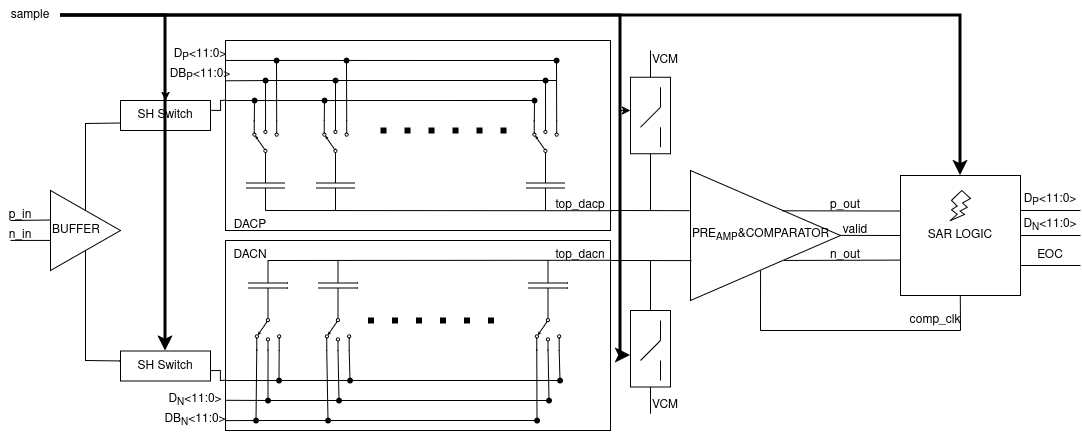
\includegraphics[width=0.8\textwidth]{figures/cadence_implement/ADC/SARADC.drawio.png}
    \caption{Fully Differential 12-bit Asynchronous SAR ADC Architecture.}
    \label{fig:adc_arch}
\end{figure}

To achieve the required linearity and speed, the ADC is composed of several critical sub-blocks, which are analyzed in detail in the following sections:

\subsection{Sample and Hold Switch}
The Sample and Hold (S/H) switch is the front-end of the ADC, responsible for acquiring the analog input signal onto the CapDAC array. To achieve high linearity over a wide input common-mode range, a bootstrapped switch topology is employed. The design is based on the well-known bootstrapped switch architecture proposed by Razavi \cite{Razavi2015}, which ensures a constant gate-to-source voltage ($V_{gs}$) for the main sampling transistor. This minimizes signal-dependent charge injection and maintains a low, constant on-resistance, which is critical for achieving 12-bit linearity.

To further enhance robustness, the bulk connections of the transistors are critical. The final implementation of the switch is shown in Figure \ref{fig:sh_switch}. The design of such high-performance switches is a well-studied area in CMOS analog design \cite{Abo1999, Razavi2015}.

\begin{figure}[H]
    \centering
    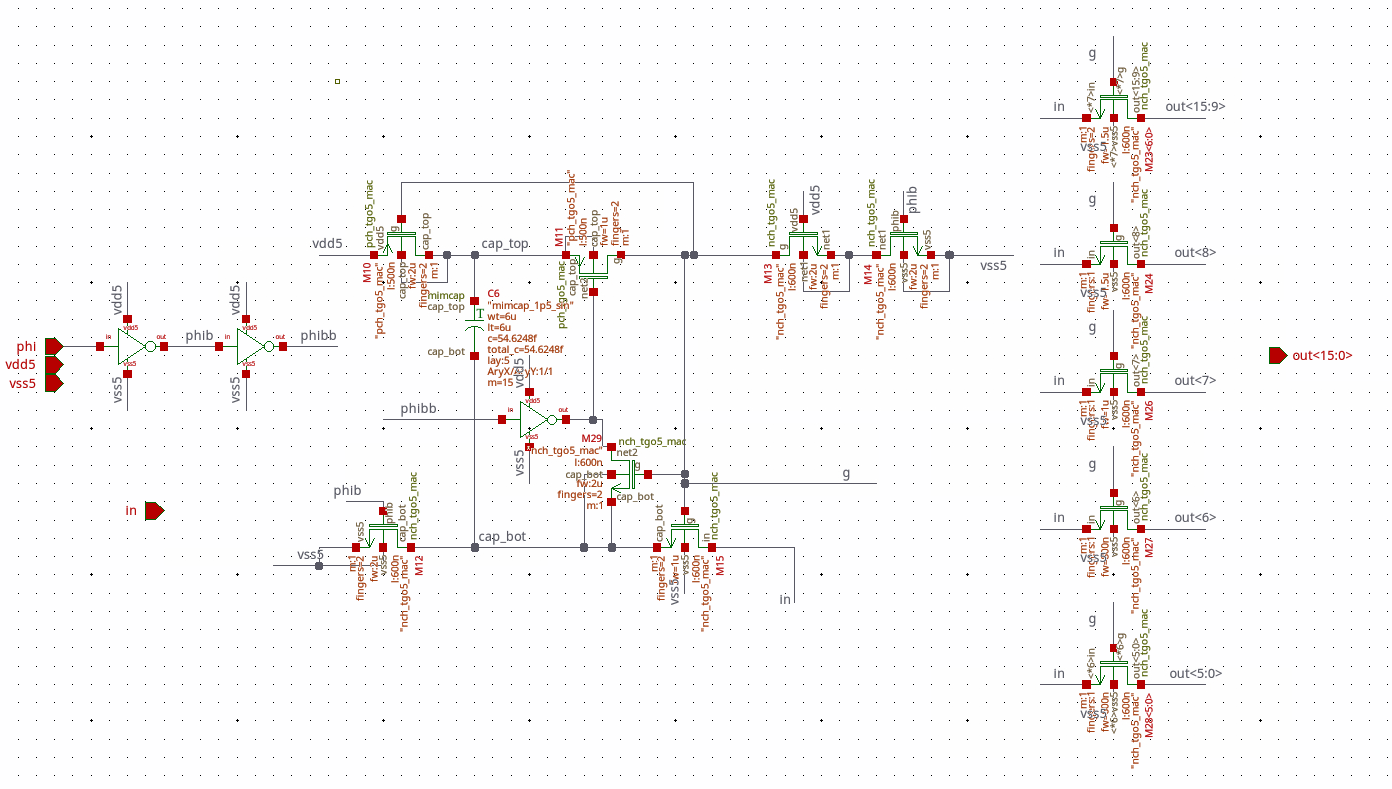
\includegraphics[width=0.7\textwidth]{figures/cadence_implement/ADC/sh/shswitch.png}
    \caption{Bootstrapped Sample and Hold Switch Implementation.}
    \label{fig:sh_switch}
\end{figure}

The parasitic capacitance on the switching node was calculated as 60 fF in the typical process corner. Consequently, a 500 fF bootstrap capacitor was selected. Although this results in a gate-source voltage ($V_{gs}$) drop of approximately 10\% due to charge sharing, the resulting on-resistance of the MOSFET is still sufficiently low to charge the $\sim$25 pF sampling capacitor within the 20 kHz sampling period.

Linearity is the main metric for this device, as any distortion introduced at the sampling stage directly limits the overall accuracy of the ADC. Figure \ref{fig:sh_dft} shows the 4096-point Discrete Fourier Transform (DFT) of the signal passed through the switch. The spectrum demonstrates the high linearity of the design, with harmonic components significantly suppressed relative to the fundamental tone.

\begin{figure}[H]
    \centering
    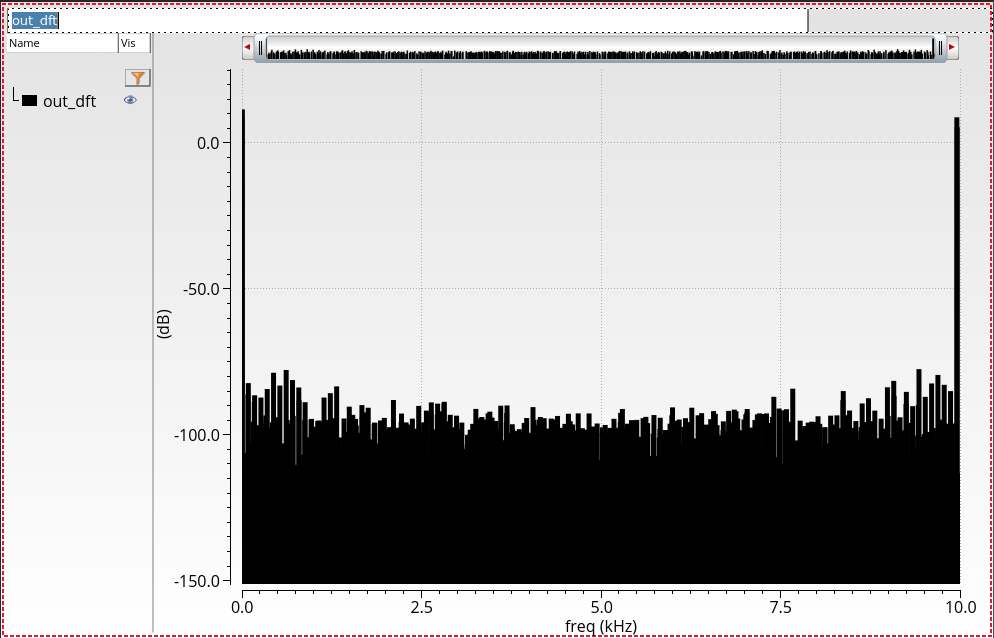
\includegraphics[width=0.8\textwidth]{figures/cadence_implement/ADC/sh/shswitchsim.png}
    \caption{DFT of the Signal Passed Through the Sample and Hold Switch.}
    \label{fig:sh_dft}
\end{figure}

\begin{table}[H]
    \centering
    \caption{Sample and Hold Switch Performance Metrics (Input: 0-5 V FS)}
    \begin{tabular}{|l|c|}
        \hline
        \textbf{Metric} & \textbf{Value} \\
        \hline
        THDB3 & -89.12 dB \\
        \hline
        SFDR & 82.2 dB \\
        \hline
    \end{tabular}
    \label{tab:sh_performance}
\end{table}

\subsection{CapDAC}
The Capacitor-DAC (CapDAC) utilizes a split-capacitor architecture to reduce the total capacitance and silicon area. Instead of a conventional $2^{12}$ unit capacitor array, the design employs a 6-bit MSB and 6-bit LSB split. Although the minimum Metal-Insulator-Metal (MIM) capacitor allowed by the PDK is 6 fF, a unit capacitor of 60 fF is used in this architecture. Following the equivalent value method described in \cite{Fan2023}, a bridge capacitor of 2C (twice the unit capacitance) was chosen, reducing the total number of unit capacitors to 128. To ensure proper binary weighting, an additional dummy capacitor is required. The calculation for this dummy capacitor was performed using the MATLAB script in Listing \ref{code:adc_split_cap}, which implements the method from \cite{Fan2023}, and resulted in a value of 62C. This configuration significantly improves the settling time and bandwidth of the ADC.

\lstinputlisting[language=MATLAB, caption={Split Capacitor Array Calculation Script}, label={code:adc_split_cap}]{matlab_code/adc_split_cap.m}

The linearity of the CapDAC is paramount for the overall ADC performance. The two key metrics are Differential Non-Linearity (DNL), which measures the deviation in step width from the ideal 1 LSB, and Integral Non-Linearity (INL), which is the cumulative sum of DNL errors. Figure \ref{fig:capdac_linearity} shows the simulated DNL and INL of the designed CapDAC.

\begin{figure}[H]
    \centering
    \subfigure[DNL]{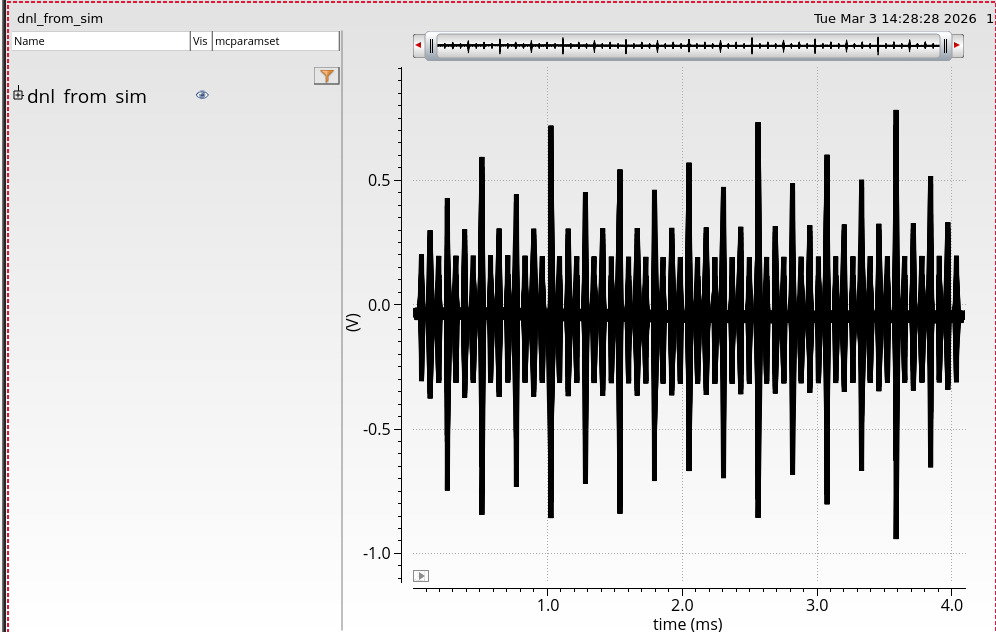
\includegraphics[width=0.8\textwidth]{figures/cadence_implement/ADC/capdac/dnlsim.png}\label{fig:capdac_dnl}}
    \vfill
    \subfigure[INL and its derivative]{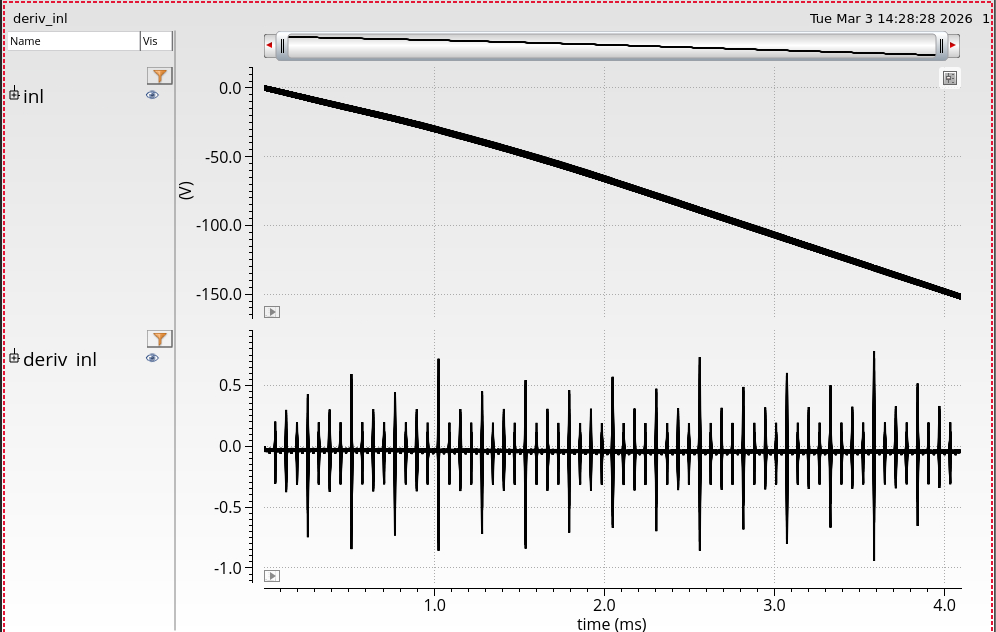
\includegraphics[width=0.8\textwidth]{figures/cadence_implement/ADC/capdac/inlandderivinl.png}\label{fig:capdac_inl}}
    \caption{CapDAC Linearity Simulation Results.}
    \label{fig:capdac_linearity}
\end{figure}

The results shown in Figure \ref{fig:capdac_linearity} are obtained from a Monte Carlo simulation of 200 runs. The Differential Non-Linearity (DNL) is observed to be up to $\pm 1$ LSB, which is a natural characteristic in split-capacitor arrays due to bridge capacitor sensitivity. However, since the target Effective Number of Bits (ENOB) for this application is 10 bits, this performance is considered acceptable. The Integral Non-Linearity (INL) is also within acceptable limits, exhibiting a nearly constant gain error. This is further illustrated by the derivative of the INL, plotted as $d(INL)/dt \times 1 \mu s$ (corresponding to the LSB step time). Finally, to further improve the ADC performance after fabrication, the bridge capacitor is implemented with trim capacitors consisting of 6 fF unit cells. Additionally, a calibration capacitance of $0.1 \times C_{unit}$ is added.

\subsection{Preamplifier}
In a high-resolution SAR ADC, the dynamic comparator can inject significant kickback noise back onto the sensitive CapDAC nodes when it fires. This charge injection can corrupt the voltage stored on the capacitor array, leading to erroneous bit decisions. To mitigate this effect and improve the overall linearity, a preamplifier is placed between the CapDAC and the comparator.

The preamplifier serves two primary functions:
\begin{enumerate}
    \item \textbf{Isolation:} It acts as a buffer, shielding the delicate analog nodes of the CapDAC from the comparator's kickback noise.
    \item \textbf{Gain:} It provides a moderate amount of voltage gain, amplifying the small differential voltage from the CapDAC. This relaxes the sensitivity requirements for the subsequent comparator, reducing its effective input-referred offset and noise.
\end{enumerate}

The implemented preamplifier, shown in Figure \ref{fig:preamp_schematic}, is a fully differential amplifier that utilizes top-plate sampling. A fully differential topology is used to maintain high common-mode noise rejection throughout the signal path. To stabilize the output common-mode voltage, which is otherwise undefined in a differential amplifier, a dedicated Common-Mode Feedback (CMFB) circuit is employed. The reference voltage for the CMFB is set to VDD/2, which is generated by a simple resistive divider filtered by a capacitor to reduce noise; this VDD/2 reference will also be used by the top-plate biasing LDO. The CMFB circuit senses the average output voltage, compares it to this reference, and adjusts the gate voltage of the PMOS load transistors to maintain a stable DC operating point.

\begin{figure}[H]
    \centering
    
\includegraphics[width=0.9\textwidth]{figures/cadence_implement/ADC/preamp/preamp.png}
    \caption{Fully Differential Preamplifier with CMFB Circuit.}
    \label{fig:preamp_schematic}
\end{figure}

\subsubsection{Simulation Results}
The performance of the preamplifier was verified through extensive simulations. The key metrics evaluated include differential and common-mode stability, input-referred offset, and noise performance.

\paragraph{CMFB Stability Analysis}
Ensuring stability is crucial for the preamplifier. The primary concern is the stability of the Common-Mode Feedback (CMFB) loop, which must be analyzed to prevent oscillations and ensure a stable output common-mode level.

\begin{figure}[H]
    \centering
    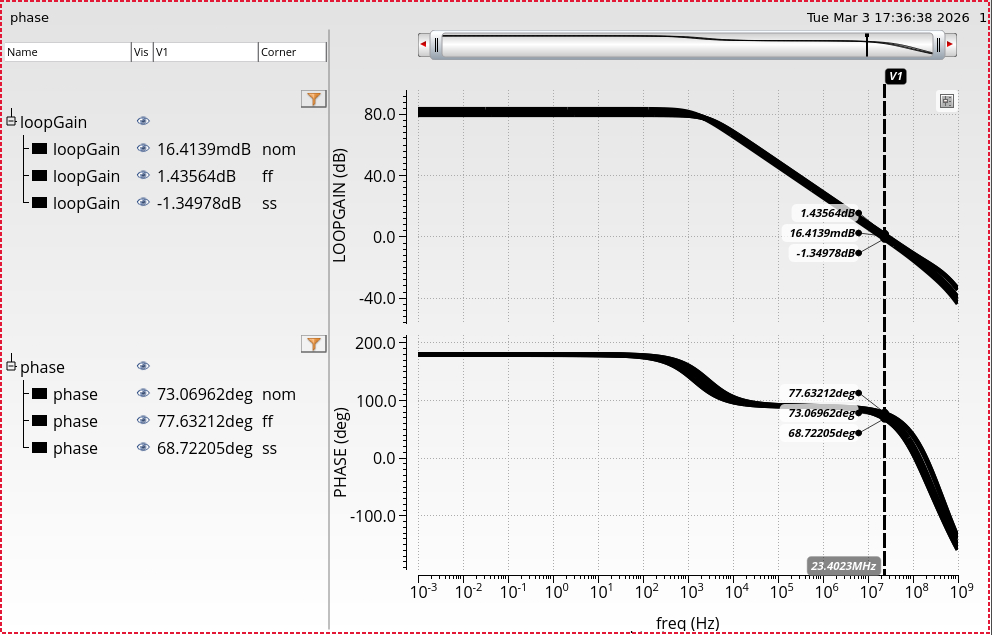
\includegraphics[width=0.8\textwidth]{figures/cadence_implement/ADC/preamp/cmfb_stb.png}
    \caption{CMFB Loop Stability Simulation.}
    \label{fig:preamp_cmfb_stb}
\end{figure}

\paragraph{Common Mode Voltage}
The output common-mode voltage is maintained by the CMFB loop. Figure \ref{fig:preamp_cm_hist} shows the Monte Carlo simulation results for the output common-mode voltage, demonstrating the effectiveness of the CMFB circuit across variations.

\begin{figure}[H]
    \centering
    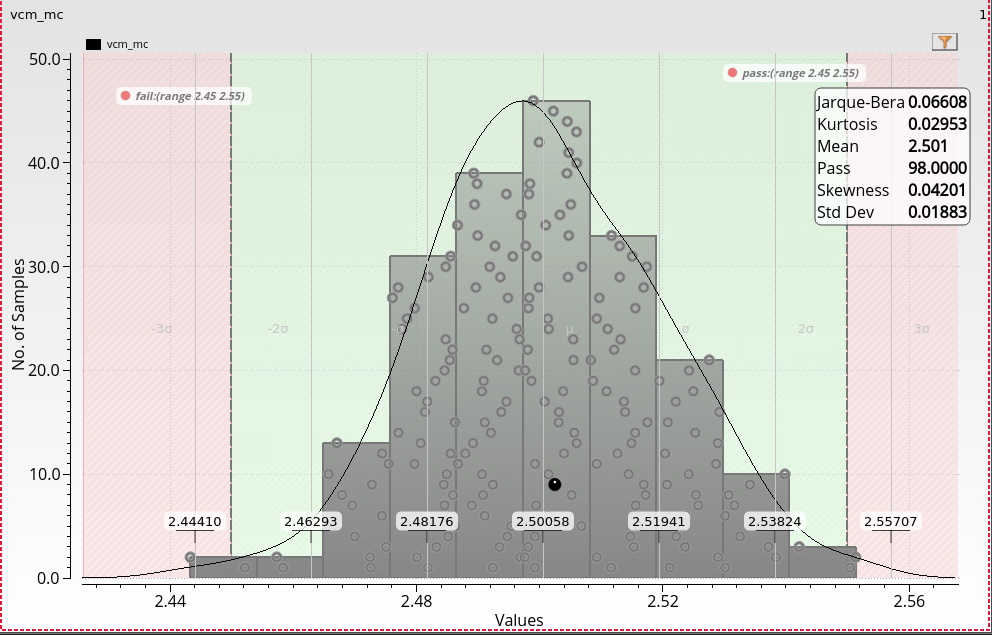
\includegraphics[width=0.8\textwidth]{figures/cadence_implement/ADC/preamp/cm_v_hist.png}
    \caption{Output Common Mode Voltage Monte Carlo Simulation.}
    \label{fig:preamp_cm_hist}
\end{figure}

\paragraph{DIFF OPEN LOOP Analysis}
The open-loop differential path is also analyzed, mainly to observe its phase delay and ensure it settles quickly without excessive ringing.

\begin{figure}[H]
    \centering
    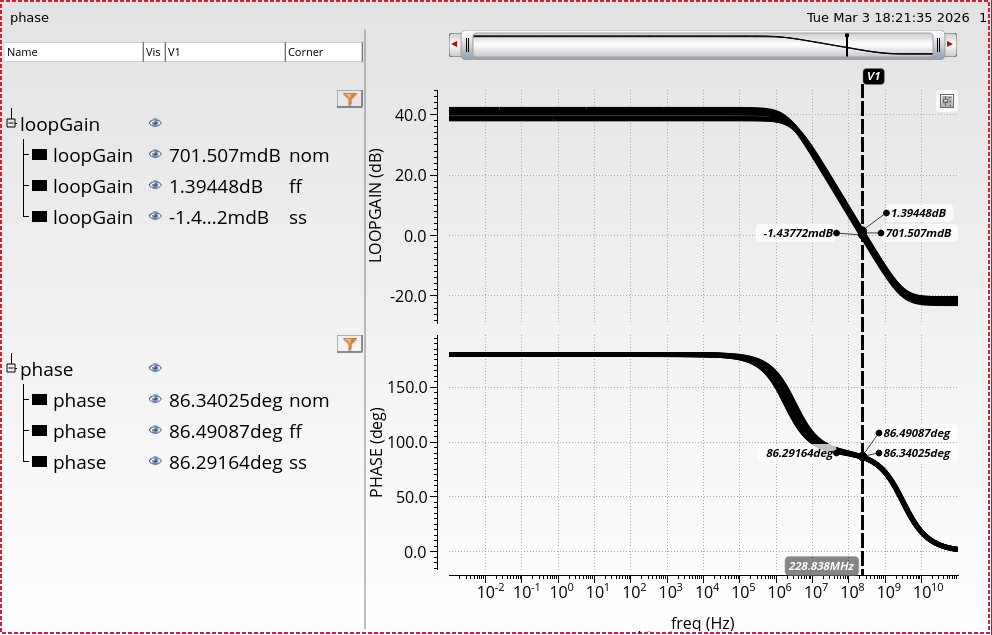
\includegraphics[width=0.8\textwidth]{figures/cadence_implement/ADC/preamp/diff_open_loop.png}
    \caption{Differential Open Loop AC Response.}
    \label{fig:preamp_diff_open}
\end{figure}

\paragraph{Offset}
The input-referred offset directly impacts the effective resolution of the ADC.

\begin{figure}[H]
    \centering
    
\includegraphics[width=0.8\textwidth]{figures/cadence_implement/ADC/preamp/offset_hist.png}
    \caption{Input Referred Offset Monte Carlo Simulation.}
    \label{fig:preamp_offset}
\end{figure}

\paragraph{Noise}
The input-referred noise is another critical factor limiting the ADC's lsb resolution. The noise is integrated up to 37 MHz and calculated as 76.97 $\mu V_{rms}$.

\begin{figure}[H]
    \centering
    
\includegraphics[width=0.8\textwidth]{figures/cadence_implement/ADC/preamp/noise_sim.png}
    \caption{Input Referred Noise Simulation.}
    \label{fig:preamp_noise}
\end{figure}

\begin{table}[H]
    \centering
    \caption{Preamplifier Performance Summary}
    \begin{tabular}{|l|c|}
        \hline
        \textbf{Parameter} & \textbf{Value} \\
        \hline
        Differential Gain & 38.7-41.8 dB \\
        \hline
        Differential Bandwidth (BW) & 1.85-3.1 MHz \\
        \hline
        Differential GBW & 228.8-269 MHz \\
        \hline
        CMFB Phase Margin & 71.7-75.43$^{\circ}$ \\
        \hline
        CMFB GBW & 20.1-27.6 MHz \\
        \hline
        Input Referred Offset ($\sigma$) & -+10 mV \\
        \hline
        Input Referred Noise (RMS) & 76.97 $\mu$V \\
        \hline
        Output Common Mode Voltage ($V_{ocm}$) & 2.45-2.55 V \\
        \hline
    \end{tabular}
    \label{tab:preamp_perf}
\end{table}

\subsection{Comparator}
The comparator is the decision-making block of the SAR ADC. To achieve high speed with zero static power consumption, a dynamic latch topology is employed. The design utilizes the StrongARM latch architecture, a widely adopted topology in low-power ADCs. The implementation incorporates the insights and modifications presented by Razavi \cite{Razavi2013} to optimize the regeneration speed and input-referred offset.

\subsubsection{Offset and Noise}
Measuring the input-referred offset is straightforward using Monte Carlo simulations to find the trip point distribution. However, for noise performance, the dynamic nature of the latch requires a specific simulation strategy. The input-referred noise was analyzed using the transient noise simulation methodology described in \cite{CadenceNoise2016}.

\begin{figure}[H]
    \centering
    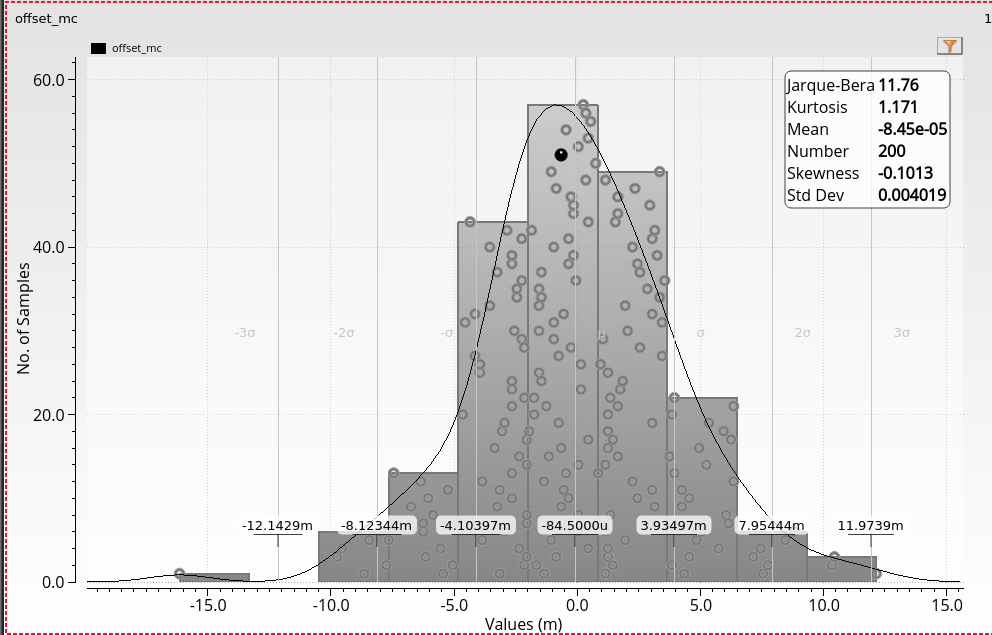
\includegraphics[width=0.8\textwidth]{figures/cadence_implement/ADC/comparator/offset_hist.png}
    \caption{Comparator Input Referred Offset Monte Carlo Simulation.}
    \label{fig:comp_offset}
\end{figure}

\begin{figure}[H]
    \centering
    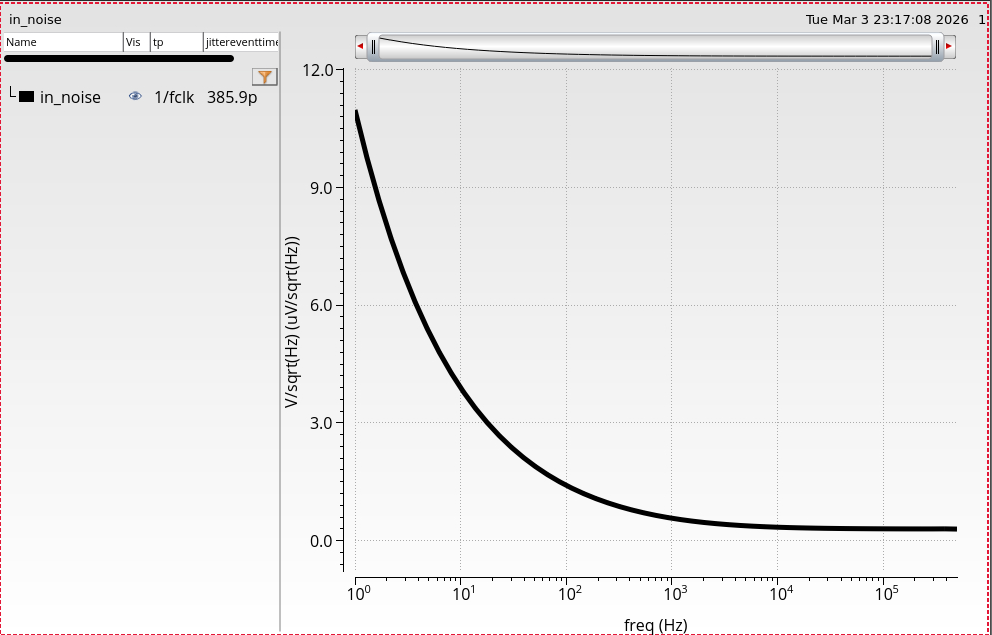
\includegraphics[width=0.8\textwidth]{figures/cadence_implement/ADC/comparator/noise_sim.png}
    \caption{Comparator Input Referred Noise Simulation.}
    \label{fig:comp_noise}
\end{figure}

\begin{table}[H]
    \centering
    \caption{Comparator Performance Summary}
    \begin{tabular}{|l|c|}
        \hline
        \textbf{Parameter} & \textbf{Value} \\
        \hline
        Input Referred Offset ($\sigma$) & -15-12 mV \\
        \hline
        Input Referred Integrated Noise (RMS) & 216 $\mu$V \\
        \hline
    \end{tabular}
    \label{tab:comp_perf}
\end{table}

It is important to note that these values are referred to the input of the comparator. Since they are divided by the gain of the preamplifier when referred to the ADC input, their impact on the overall system performance is significantly reduced and considered negligible.

\subsection{SAR Logic}
The Successive Approximation Register (SAR) logic is the digital core that orchestrates the binary search algorithm. To maximize operation speed and avoid the need for a high-frequency oversampling clock, the logic is implemented using an asynchronous topology. The internal state transitions are self-timed, triggered by the ready signal from the comparator rather than a global clock edge.

The system operates across two voltage domains. The analog front-end, including the switches and capacitor array, operates at the 5V I/O voltage to maximize the signal-to-noise ratio. However, the complex digital logic is implemented using 1V core transistors to reduce dynamic power consumption and silicon area. Consequently, the comparator output is level-shifted down to 1V before being processed by the SAR engine. The resulting control signals are then level-shifted back up to 5V to drive the CapDAC switches.

\begin{figure}[H]
    \centering
    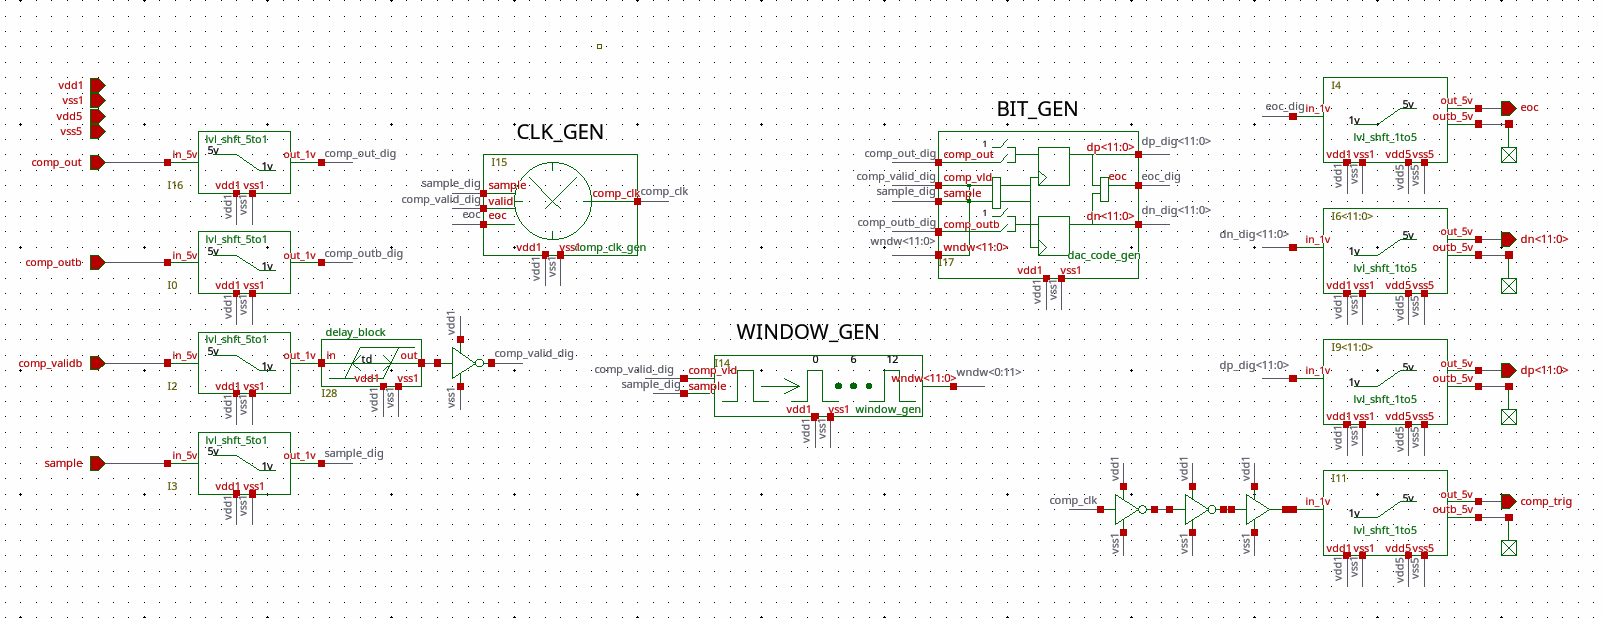
\includegraphics[width=0.8\textwidth]{figures/cadence_implement/ADC/sar_logic/sar_logic_overview.png}
    \caption{Asynchronous SAR Logic Overview with Level Shifters.}
    \label{fig:sar_logic_overview}
\end{figure}

\subsubsection{Window Generator}
The window generator is responsible for orchestrating the timing of the bit trials. It generates 12 distinct window outputs, corresponding to the 12 bits of resolution. These signals are mutually exclusive; only one window bit is high at any given instance, indicating the specific bit currently being processed. This ensures the sequential operation of the SAR algorithm.

\begin{figure}[H]
    \centering
    
\includegraphics[width=0.8\textwidth]{figures/cadence_implement/ADC/sar_logic/window_gen.png}
    \caption{Window Generator Logic Implementation.}
    \label{fig:window_gen}
\end{figure}

\subsubsection{Comparator Clock Generator}
The comparator clock is generated asynchronously to maximize speed and eliminate the need for a high-frequency external clock. The process initiates with the sampling signal, which triggers the first clock pulse. Subsequent clock pulses are self-timed; they are generated upon the receipt of a 'valid' signal from the comparator, indicating that a decision has been made. This loop continues, generating a new clock edge for each bit trial, until the End of Conversion (EOC) signal is asserted, which inhibits further clock generation. Ideally, the EOC signal should directly reset the flip-flops to minimize power consumption, but this optimization was not implemented.

\begin{figure}[H]
    \centering
    
\includegraphics[width=0.8\textwidth]{figures/cadence_implement/ADC/sar_logic/comp_clk_gen.png}
    \caption{Asynchronous Comparator Clock Generation Logic.}
    \label{fig:comp_clk_gen}
\end{figure}

A potential enhancement for this architecture is the implementation of adaptive clock timing. Generally, the MSB capacitors in the DAC require a longer settling time compared to the LSB capacitors due to the larger voltage steps and stricter accuracy requirements. Conversely, the LSBs settle much faster. By leveraging the window bits, which track the current conversion step, the system can dynamically select different delay paths within the clock generation loop. This approach allocates more time for MSB decisions and speeds up LSB decisions, thereby optimizing the total conversion time. The bottom half of the circuit can be easily modified to implement this, but it is not necessary. To better illustrate the timing of the asynchronous operation, a simplified timing diagram is provided in Figure \ref{fig:sar_timing}.

\begin{figure}[H]
    \centering
    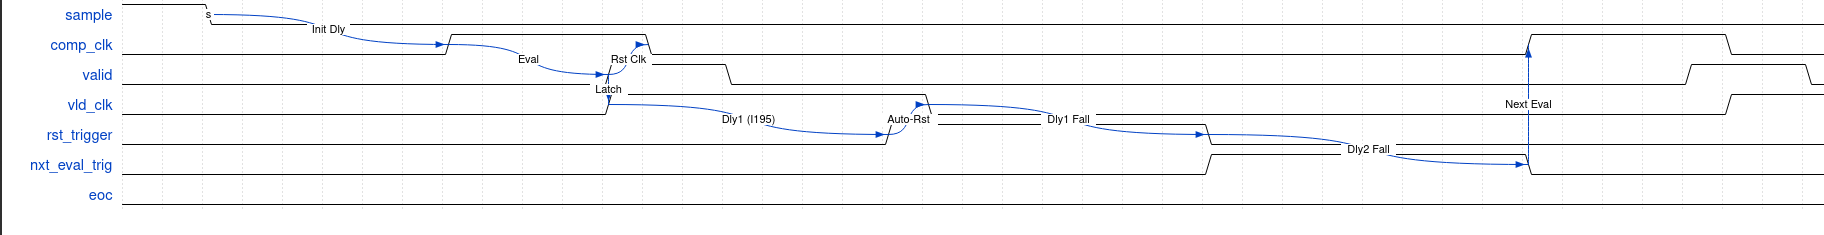
\includegraphics[width=0.8\textwidth]{figures/cadence_implement/ADC/sar_logic/timing_diagram.png}
    \caption{Timing Diagram of the Asynchronous Operation.}
    \label{fig:sar_timing}
\end{figure}

\subsubsection{Bit Generator}
The bit generator controls the sequential switching of the capacitor array, moving from the MSB to the LSB. There are no special design intricacies for this block; a direct set-and-down logic is implemented.

\begin{figure}[H]
    \centering
    
\includegraphics[width=0.8\textwidth]{figures/cadence_implement/ADC/sar_logic/bit_gen.png}
    \caption{Bit Generator Logic Implementation.}
    \label{fig:bit_gen}
\end{figure}

\subsection{ADC Top-Level Performance}
The overall performance of the 12-bit SAR ADC was evaluated, considering the impact of noise, linearity, and process variations.

Given the 5V input range, the LSB size is approximately 1.22 mV. The combined input-referred noise from the preamplifier and comparator is significantly lower than the quantization noise level. Consequently, the system is not noise-limited, and the 12-bit resolution is not compromised by thermal noise.

The primary source of error is the Differential Non-Linearity (DNL) arising from the split-capacitor DAC array. As previously discussed, the DNL can approach $\pm 1$ LSB. However, since the target Effective Number of Bits (ENOB) for this application is 10 bits, this linearity performance is considered acceptable. Nevertheless, as a precautionary measure to further minimize DNL errors, calibration capacitances were incorporated around the bridge capacitor.

Regarding the offset voltage introduced by the preamplifier and comparator, its impact on the MPPT algorithm is minimal. The system operates in a relatively slow-changing environment (solar irradiance and temperature), and the control logic relies primarily on the differential changes in voltage ($dV$) and current ($dI$) rather than absolute precision. Since the offset appears as a constant DC error across consecutive samples, it cancels out during the differential calculation, ensuring that the tracking direction remains accurate.

Figure \ref{fig:adc_fft} presents the 4096-point FFT of the ADC output, illustrating the dynamic performance. The analysis was performed using a Blackman-Harris window with a sampling frequency of 20 kSPS. The input frequency was chosen as $f_{in} = \frac{2039}{4096} f_s$, placing it close to the Nyquist frequency. The input signal was a differential sinusoid with a differential peak-to-peak swing of $\pm 8$ V. For the dynamic performance calculations, the peak saturation level was set to 5 V, and the first 10 harmonics were considered.

For the Slow-Slow (ss) and Fast-Fast (ff) process corners, a 256-point FFT was utilized. The primary purpose of this analysis was to verify the functional robustness of the asynchronous logic and to confirm that process variations do not cause timing issues, rather than to obtain high-precision dynamic performance metrics. Table \ref{tab:adc_corners} summarizes the key performance metrics across different process corners.

\begin{figure}[H]
    \centering
    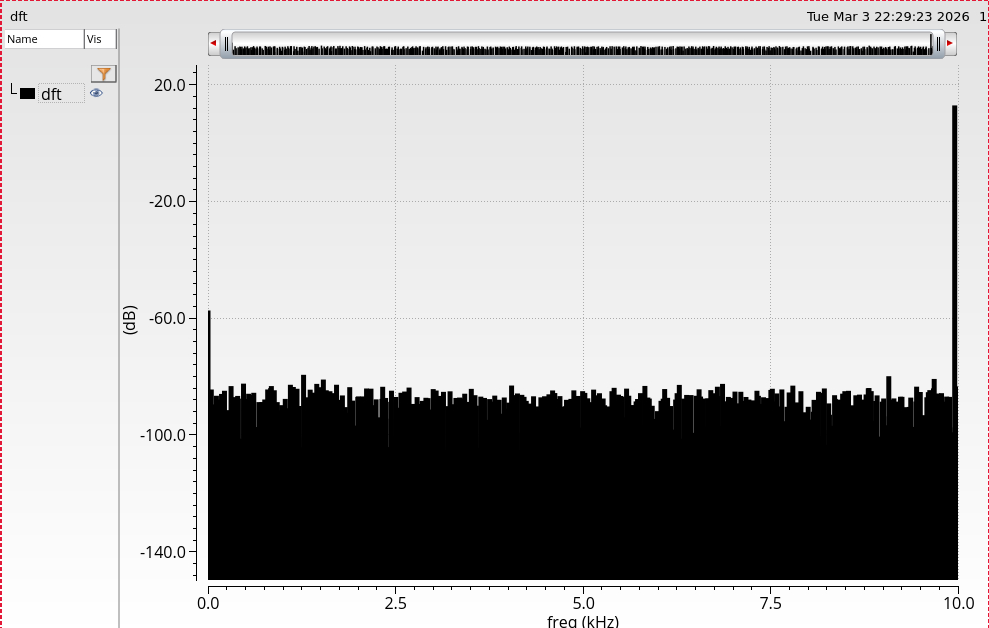
\includegraphics[width=0.8\textwidth]{figures/cadence_implement/ADC/adc_fft.png}
    \caption{4096-Point FFT of the ADC Output.}
    \label{fig:adc_fft}
\end{figure}

\begin{table}[H]
    \centering
    \caption{ADC Performance Across Process Corners}
    \begin{tabular}{|l|c|c|c|c|}
        \hline
        \textbf{Corner} & \textbf{SFDR (dB)} & \textbf{SNR (dB)} & \textbf{SINAD (dB)} & \textbf{ENOB (bits)} \\
        \hline
        Typical (tt) & 98.12 & 72.03 & 72 & 11.99 \\
        \hline
        Slow-Slow (ss) & 88.18 & 68.91 & 70.53 & 11.96  \\
        \hline
        Fast-Fast (ff) & 87.6 & 69.36 & 70.89 & 12.02 \\
        \hline
    \end{tabular}
    \label{tab:adc_corners}
\end{table}

\section{DAC}
The digital-to-analog converter used in the system.
% Add more details here.

\section{LDO}
The Low-Dropout regulator design and implementation.
% Add more details here.

\section{Duty Cycle Generator}
The circuit for generating the duty cycle for the buck converter.
% Add more details here.

\chapter{DIGITAL IMPLEMENTATION}
\label{chapter:digital_impl}

\section{Fuzzy Logic}
A detailed description of the digital implementation of the fuzzy logic controller.
% Add more details here.

\section{SPI Interface}
The implementation of the Serial Peripheral Interface (SPI) for communication will be detailed here.
% Add more details here.


\chapter{CONCLUSION}
\label{chapter:conclusion}
The conclusions of the thesis should come here.

\nocite{*}
\bibliographystyle{styles/fbe_tez_v11.bst}
\bibliography{references}

\appendix
\chapter{APPENDIX A}
\label{appendix:a}
This is the first appendix.

\end{document}
